\documentclass[aps,twocolumn,secnumarabic,nobalancelastpage,amsmath,amssymb,
nofootinbib,superscriptaddress]{revtex4-1}

\usepackage{graphics}       % standard graphics specifications
\usepackage{graphicx}       % alternative graphics specifications
\usepackage{longtable}      % helps with long table options
\usepackage{url}            % for on-line citations
\usepackage{bm}             % special 'bold-math' package
\usepackage[ngerman]{babel} % deutsche Siblentrennung
\usepackage[utf8]{inputenc} % Umlaute
\usepackage{chemformula}    % für chemische Schreibweise
\usepackage{lipsum}

\def\andname{\hspace*{-0.5em},} % definiert die Trennung zwischen 2 Autoren neu

% Titelseite
\begin{document}
\title{F-Praktikum (Phasendiagramme):\\Differentialthermoanalyse von $\text{TbGdScO}_3$
und $\text{DyTbScO}_3$\\im Bereich zwischen 300 K und 2500 K}
\author         {Ch. Egerland}
\email[Email: ]{egerlanc@physik.hu-berlin.de}
\author         {M. Pfeifer}
\email[Email: ]{max.pfeifer@physik.hu-berlin.de}
\affiliation    {Humboldt-Universität zu Berlin, Institut für Physik}
\date[Versuchsort: ]{Leibniz-Institut für Kristallzüchtung \\ VVVersuchsdatum: 05.09.2017}

%%%%%%%%%%%%%%%%%%%%%%%%%%%%%%%%%%%%%%%%%%%%%%%%%%%%%%%%%%%%%%%%%%%%%%%%%%%%%%%%

\begin{abstract}
Mischkristalle aus Skandat ($\text{ScO}_3$) und einem seltenen Erdelement (RE), auch $\text{REScO}_3$ bzw. RE-Skandate, finden heutzutage häufig Anwendung bei der Herstellung
dünner Perowskit-Filme. Dies ist der Tatsache geschuldet, dass $\text{REScO}_3$ Gitterparameter im Bereich von 3.95 \AA$\text{ bis}$ 4.02 \AA$\text{ aufweisen.}$
 Untersucht wird das Temperaturverhalten der Mischkristalle $\text{TbGdScO}_3$ und $\text{DyTbScO}_3$ mittels
Differentialthermoanalyse zur näherungsweisen Bestimmung der Schmelzwärmen ($\Delta Q_S=20\text{ }\%$) sowie Schmelztemperaturen ($\Delta T_S=20\text{ K}$).
Die genannten Verbindungen werden anschließend in die Systematik der Mischbarkeit von Phasen eingeordnet (XXXXXXXX ES HANDELT SICH UM ... SYSTEM).
Basierend auf Referenzdaten zu $\text{Gd}\text{ScO}_3$ und $\text{Dy}\text{ScO}_3$ aus \cite{paperK} werden die Schmelzwärmen und -temperaturen dieser
reinen RE-Skandate mit denen der hier untersuchten Materialien verglichen.
\end{abstract}


\maketitle

%%%%%%%%%%%%%%%%%%%%%%%%%%%%%%%%%%%%%%%%%%%%%%%%%%%%%%%%%%%%%%%%%%%%%%%%%%%%%%%%
%%%%%%%%%%%%%%%%%%%%%%%%%%%%%%%%%%%%%%%%%%%%%%%%%%%%%%%%%%%%%%%%%%%%%%%%%%%%%%%%
%%%%%%%%%%%%%%%%%%%%%%%%%%%%%%%%%%%%%%%%%%%%%%%%%%%%%%%%%%%%%%%%%%%%%%%%%%%%%%%%

\section{Theorie}
\subsection{Struktur und Eigenschaften von $\text{REScO}_3$}
\noindent Skandate spielen in der Forschung wegen ihrer speziellen Kristallstruktur und aufgrund der Anpassbarkeit bestimmter Gittereigenschaften, wie z.B. der
Gitterparameter, eine entscheidene Rolle. $\text{REScO}_3$ mit $\text{RE=Pr, Nd, Pm, Sm, Eu, Gd, Tb, Dy}$, sowie $\text{NdSmScO}_3$ und $\text{SmGdScO}_3$ wurden bereits untersucht \cite{paperK}.
Dabei fällt der Gitterparameter des Mischkristalls mit steigender Ordnungszahl des RE-Elements näherungsweise in 0.01 \AA-Schritten. \cite{paperK}

Jedoch sind nicht alle seltenen Erden als Bestandteil von RE-Skandaten geeignet ($\text{PmScO}_3$ radioaktiv, $\text{EuScO}_3$ instabil bei Kontakt mit Si).
Weiterhin kristallisieren nicht alle RE-Skandate in der Perowskit-Struktur. Nach \cite{perowskHoPr} kann jedoch davon ausgegangen werden, dass solche $\text{REScO}_3$ mit
$\text{RE}=\ch{_{57}Pr}$ bis $\ch{_{67}Ho}$ isomorph sind. Im Gegensatz zur idealerweise kubischen Perowskitstruktur, besitzen diese eine orthorhombische Kristallstruktur.

Um die als Kristallbestandteil ungeeigneten Lanthanoide zu ersetzen, werden auf Grundlage der Vergardschen Regel Mischkristalle aus jeweils benachbarten RE-Skandaten gezüchtet so z.B.
$\text{Sm}_x\text{Gd}_{1-x}\text{ScO}_3$ für $\text{EuScO}_3$ oder $\text{Nd}_x\text{Sm}_{1-x}\text{ScO}_3$ für $\text{PmScO}_3$ \cite{paperK}. Werden Mischkristalle gezüchtet,
die neben $\text{ScO}_3$ zwei direkt benachbarte seltene Erdelemente enthalten ($\ch{^{x}RE^{y}REScO_3}$, wobei $|x-y|=2$) ist eine gezieltere Feinabstimmung gewünschter
Film-Eigenschaften (z.B. Anpassung Gitterparameter in der Größenordnung von 0.002 \AA$\text{ statt }$ 0.01 \AA$\text{ mit}$ reinen RE-Skandaten) möglich. Dazu werden in diesem Versuch
die Verbindungen $\text{Tb}_{0.5}\text{Gd}_{0.5}\text{ScO}_3$ und $\text{Dy}_{0.5}\text{Tb}_{0.5}\text{ScO}_3$ mittels Differentialthermoanalyse untersucht.

\subsection{Differentialthermoanalyse (DTA)}
\begin{figure}[b]
  \centering
  \includegraphics[width=0.48\textwidth]{../img/exp.jpg}
  \caption{\label{fig:exp} Prinzip der Differentialthermoanalyse. \textbf{R} - Referenz, \textbf{P} - Probe, \textbf{O} - Ofen. Aus \cite{versuchsbeschr}}
\end{figure}

\noindent Die DTA ist ein thermisches Untersuchungsverfahren zur Materialanalyse. Dabei befindet sich innerhalb eines evakuierten Ofens ein hochtemperaturbeständiger Tiegelhalter
mit zwei symmetrischen Schmelztiegeln: ein Probentiegel und ein leerer (oder mit einer inerten Substanz gefüllten) Referenztiegel. An jedem Probentiegel ist,
wie in Abb. \ref{fig:dtaDyTb+TbGd} zu erkennen, jeweils ein Thermoelement befestigt. Wird der Ofen geheizt, entsteht aufgrund des Seebeck-Effektes eine zur Temperatur proportionale Spannung zwischen den Drahtenden.

Findet im Probentiegel nun ein Phasenübergang statt, der Umwandlungswärme benötigt (1. Art), so steigt die Temperatur dort langsamer an als am Referenztiegel. Durch Reihenschaltung beider
Thermoelemente kann diese Differenzspannung/-temperatur (Größenordnung 20 $\text{µV}$) direkt gemessen werden. Nimmt man zusätzlich die absolute Temperatur am Referenztiegel auf, können materialspezifische Eigenschaften
der Probensubstanz, wie Schmeltemperatur und -wärme (Peakfläche) bestimmt werden.


%%%%%%%%%%%%%%%%%%%%%%%%%%%%%%%%%%%%%%%%%%%%%%%%%%%%%%%%%%%%%%%%%%%%%%%%%%%%%%%%
%%%%%%%%%%%%%%%%%%%%%%%%%%%%%%%%%%%%%%%%%%%%%%%%%%%%%%%%%%%%%%%%%%%%%%%%%%%%%%%%
%%%%%%%%%%%%%%%%%%%%%%%%%%%%%%%%%%%%%%%%%%%%%%%%%%%%%%%%%%%%%%%%%%%%%%%%%%%%%%%%

\begin{figure}[t]
  \centering
   \includegraphics[width=0.48\textwidth]{../img/Messkurven_unsere.png}
  \caption{\label{fig:dtaDyTb+TbGd} DTA von $\text{Al}_{2}\text{O}_3$ (grün), $\text{Dy}_{0.5}\text{Tb}_{0.5}\text{ScO}_3$ (rot)
  und $\text{Tb}_{0.5}\text{Gd}_{0.5}\text{ScO}_3$ (blau); unkorrigierte Temperaturskala ($\text{T}_{korr}=T + 198\text{ °C}$)}
\end{figure}

\section{Experiment}
\noindent Die Messung wird im Leibniz-Institut für Kristallzüchtung (IKZ) mit der DTA-Messaparatur \texttt{STA 429} von der Firma \texttt{NETZSCH} durchgeführt. Die Steuerungssoftware
\texttt{Measurement Program STA 409 CD (Netzsch)} übernimmt neben dem Evakuieren des Ofens das zeitlineare Heizen (Heizrate 15 K/min) und die Aufnahme der zeitabhängigen Differenzthermospannung.
Damit keine Oxidation der Proben stattfindet, finden alle Messungen unter He-Atmosphäre statt. Die Schmelztiegel bestehen aufgrund der hohen
Temperaturbeständigkeit aus reinem Wolfram. Das Thermoelement setzt sich aus Wolfram und Rhenium (Schmelzpunkte 3.422 °C und 3.186 °C) zusammen.
Untersucht werden 62,85 mg $\text{Dy}_{0.5}\text{Tb}_{0.5}\text{ScO}_3$ und 72,75 mg $\text{Tb}_{0.5}\text{Gd}_{0.5}\text{ScO}_3$, wobei die Differenzspannung jeweils
einmal im Temperaturbereich zwischen 24 °C und 2200 °C und ein weiteres mal im Bereich zwischen 500 °C und 2200 °C gemessen wird. Eine weitere DTA
mit $\text{Al}_2\text{O}_3$, dessen Schmelzpunkt und -wärme bekannt ist ($T_S=2054\text{ °C}$, $Q_S=118.4\text{ kJ/mol}$), gewährleistet die Kalibrierung der gemessenen Temperatur
und der Wärmemenge (integrierte DTA-Peaks).


%%%%%%%%%%%%%%%%%%%%%%%%%%%%%%%%%%%%%%%%%%%%%%%%%%%%%%%%%%%%%%%%%%%%%%%%%%%%%%%%
%%%%%%%%%%%%%%%%%%%%%%%%%%%%%%%%%%%%%%%%%%%%%%%%%%%%%%%%%%%%%%%%%%%%%%%%%%%%%%%%
%%%%%%%%%%%%%%%%%%%%%%%%%%%%%%%%%%%%%%%%%%%%%%%%%%%%%%%%%%%%%%%%%%%%%%%%%%%%%%%%

\section{Daten und Analyse}
\noindent Mithilfe der Analysesoftware \texttt{Proteus Thermal Analysis} lässt sich die auf die jeweilige Probenmasse normierte Differenzspannung in
Abhängigkeit von der Temperatur darstellen. Außerdem wird der Schmelzpunkt durch die Onset-Temperatur (Schnittpunkt Wendetangente mit Basislinie) \cite{versuchsbeschr} und die Schmelzwärme (Peakfläche)
berechnet. Die temperaturabhängigen DTA-Messkurven für $\text{Dy}_{0.5}\text{Tb}_{0.5}\text{ScO}_3$, $\text{Tb}_{0.5}\text{Gd}_{0.5}\text{ScO}_3$ und $\text{Al}_{2}\text{O}_3$ sind in Abb. \ref{fig:dtaDyTb+TbGd} dargestellt.

Zunächst sind bei allen Substanzen Phasenübergänge zu erkennen. Auffällig ist, dass bei jeder zweiten Messung die Onset-Temperatur systematisch hin zu kleineren Temperaturen verschoben ist (Größenordnung 20-25 °C).
Dies wurde auch bei früheren Messungen, jedoch mit geringerer Abweichung (ca. 10 °C) an $\text{GdScO}_3$ und $\text{DyScO}_3$ festgestellt.

Da pro Substanz nur zwei Messwerte für Schmelzpunkt und -wärme vorliegen ($\text{Al}_2\text{O}_3$ nur eine Messung), werden die Unsicherheiten mit $\Delta T_S=20\text{ K}$ und $\Delta Q_S=0,2\cdot Q_S$ abgeschätzt.
Die Peakflächen wurden aufgrund unterschiedlicher molarer Massen zunächst von µVs/mg in µVs/mol umgerechnet und dann zur bekannten Schmelzwärme von $\text{Al}_2\text{O}_3$ ins Verhältnis gesetzt.

Es ergeben sich folgende Werte:
\begin{eqnarray}
  \text{TbGdScO}_3:\;\;\;\;\; T_S = (2149\,\pm\, 20)\text{ °C}\;\:\,\;\;\;\;\;\:\: \nonumber \\
  Q_S = (142\,\pm\, 28)\text{ kJ/mol}            \;\;\;             \nonumber \\
                                                        \;\;\;               \nonumber \\
  \text{DyTbScO}_3:\;\;\;\;\; T_S = (2114\,\pm\, 20)\text{ °C}\;\:\,\;\;\;\;\;\:\: \nonumber \\
  Q_S = (163\,\pm\, 33)\text{ kJ/mol}                     \;\;\;             \nonumber
  \label{eq:XXX}
\end{eqnarray}

\noindent Zum Vergleich der Ergebnisse sind in Abb. \ref{fig:dtaAll} zusätzlich die DTA-Kurven vorangegangener Messungen von $\text{GdScO}_3$ und $\text{DyScO}_3$ dargestellt.
Die Daten wurden von Herrn Dr. D. Klimm vom IKZ bereitgestellt.

\begin{figure}[h]
  \centering
   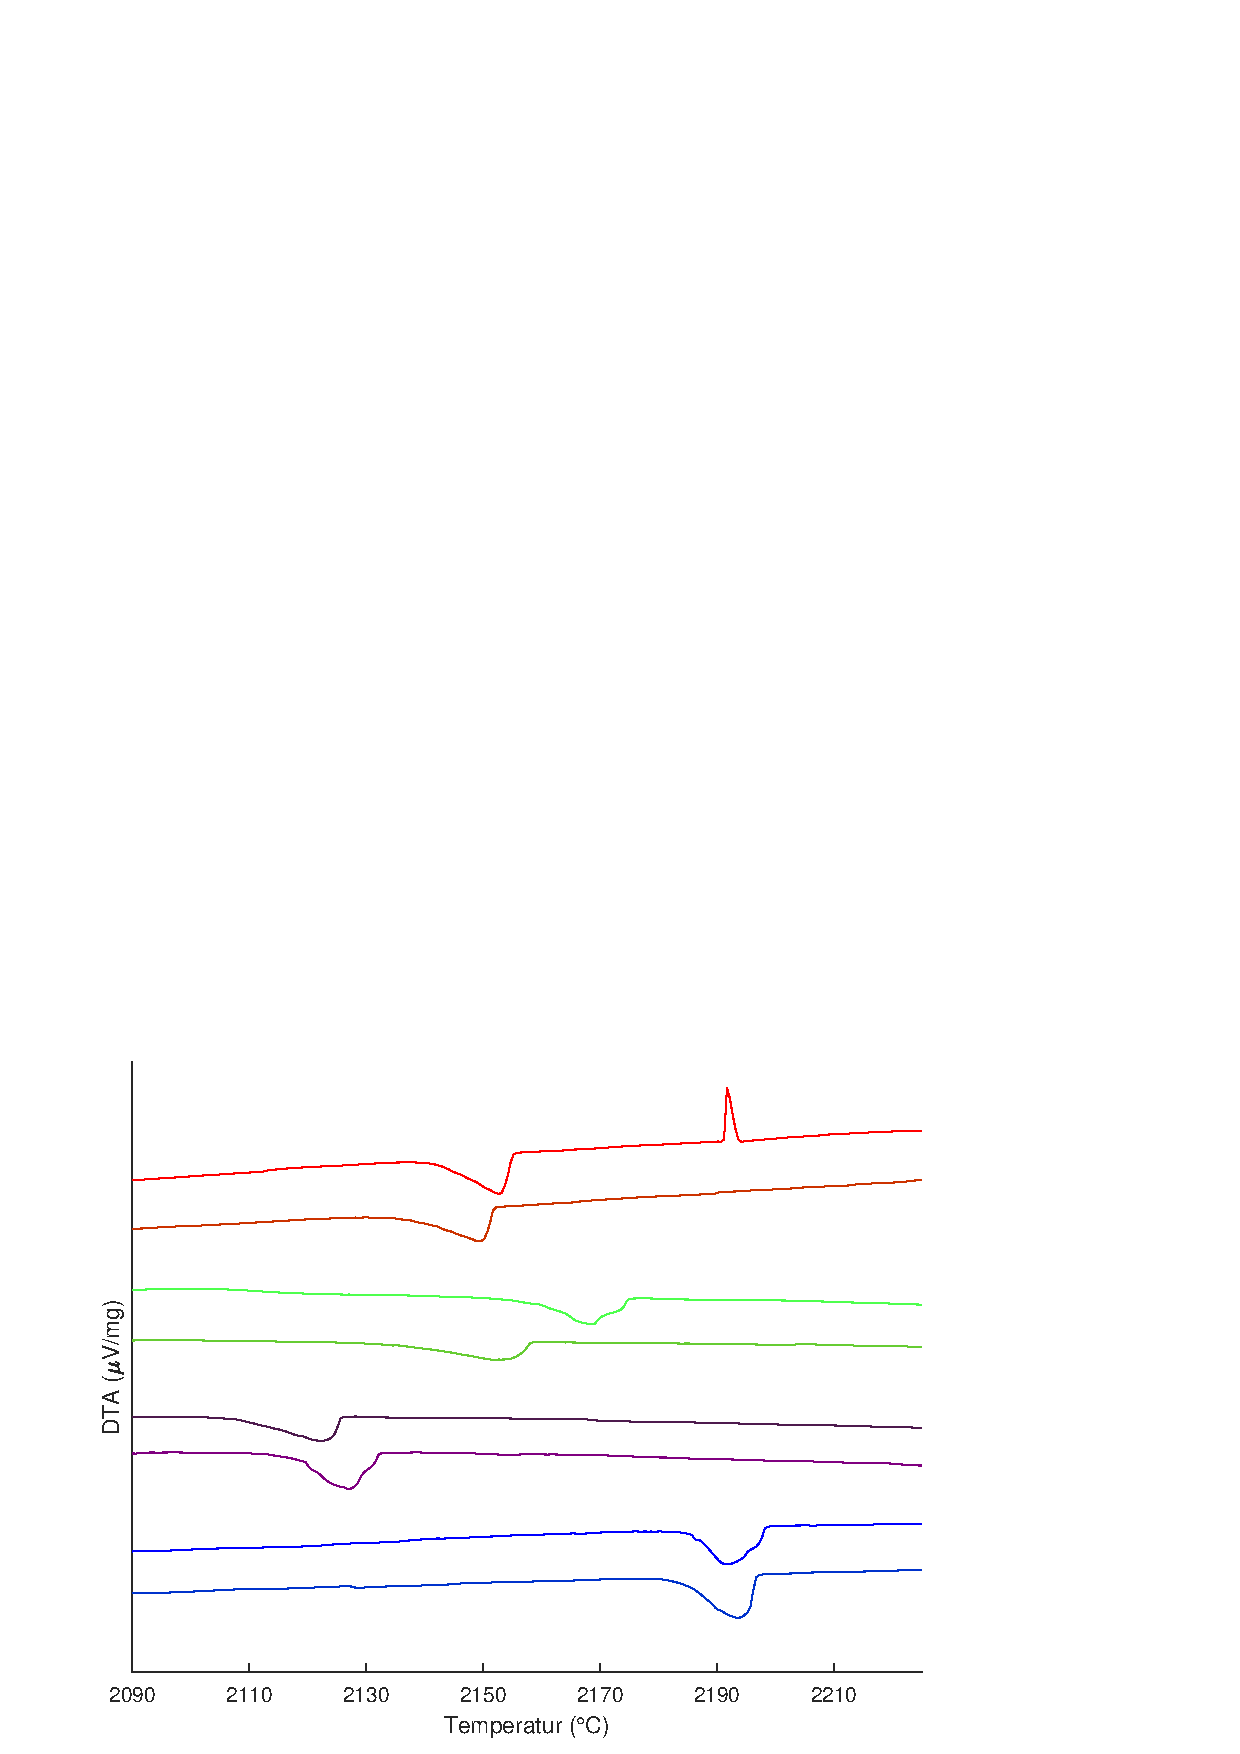
\includegraphics[width=0.48\textwidth]{../img/vglSkandate.jpg}
  \caption{\label{fig:dtaAll} DTA von $\text{GdScO}_3$, $\text{GdTbScO}_3$, $\text{TbDyScO}_3$ und $\text{DyScO}_3$ (v.o.n.u.) }
\end{figure}

Offensichtlich findet zwischen 2110 °C und 2210 °C bei allen Proben ein Phasenübergang erster Ordnung statt. Sy

\begin{figure}[h]
  \centering
   \includegraphics[width=0.48\textwidth]{../img/plotSchmelzwaermen.jpg}
  \caption{\label{fig:QAll} Schmelzwärmen von $\text{GdScO}_3$, $\text{GdTbScO}_3$, $\text{TbDyScO}_3$ und $\text{DyScO}_3$ (v.l.n.r.) }
\end{figure}

%%%%%%%%%%%%%%%%%%%%%%%%%%%%%%%%%%%%%%%%%%%%%%%%%%%%%%%%%%%%%%%%%%%%%%%%%%%%%%%%
%%%%%%%%%%%%%%%%%%%%%%%%%%%%%%%%%%%%%%%%%%%%%%%%%%%%%%%%%%%%%%%%%%%%%%%%%%%%%%%%
%%%%%%%%%%%%%%%%%%%%%%%%%%%%%%%%%%%%%%%%%%%%%%%%%%%%%%%%%%%%%%%%%%%%%%%%%%%%%%%%

\section{Schlussfolgerungen}

\noindent


%%%%%%%%%%%%%%%%%%%%%%%%%%%%%%%%%%%%%%%%%%%%%%%%%%%%%%%%%%%%%%%%%%%%%%%%%%%%%%%%
%%%%%%%%%%%%%%%%%%%%%%%%%%%%%%%%%%%%%%%%%%%%%%%%%%%%%%%%%%%%%%%%%%%%%%%%%%%%%%%%
%%%%%%%%%%%%%%%%%%%%%%%%%%%%%%%%%%%%%%%%%%%%%%%%%%%%%%%%%%%%%%%%%%%%%%%%%%%%%%%%

\bibliography{sample-paper}
\bibliographystyle{prsty}
\begin{thebibliography}{99}
\bibitem{paperK}R. Uecker, D. Klimm, R. Bertram, M. Bernhagen, I. Schulze-Jonack, M. Brützam et al., Acta Physica Polonica A, Vol. 124 [2013]
\bibitem{versuchsbeschr}Versuchsbeschreibung F-Praktikumsversuch "Phasendiagramme", Dr. D. Klimm, Leibniz-Institut für Kristallzüchtung [2016]
\bibitem{meltpDyScO3}Crnogorac, H. Wilke, Measurement of physical properties of DyScO3 melt, Vol. 44, I 6 [2009]
\bibitem{meltpDyGdScO3}B. Velickov, V. Kahlenberg, R. Bertram, M. Bernhagen, Z. Kristallogr. 222, p 466-473 [2007]
\bibitem{schmelzwAl2O3}Zhang, P.H., Chang, R.Z., Wei, Z. et al., Int J Thermophys 7: 811. [1986]
\bibitem{schmelzwAl2O3_2}Dale L. Perry, Sidney L. Phillips, Inorganic Compounds, CRC Press, p 10 [1995]
\bibitem{perowskHoPr}V.M. Goldschmidt, Naturwissenschaften 14, 477 [1926]
\end{thebibliography}

%%%%%%%%%%%%%%%%%%%%%%%%%%%%%%%%%%%%%%%%%%%%%%%%%%%%%%%%%%%%%%%%%%%%%%%%%%%%%%%%

\clearpage
\appendix

%%%%%%%%%%%%%%%%%%%%%%%%%%%%%%%%%%%%%%%%%%%%%%%%%%%%%%%%%%%%%%%%%%%%%%%%%%%%%%%%

\end{document}
